%!TEX root = ../main.tex

\section{Approach}
\label{sec:mathematical_formulation}

We formulate our drone race optimization problem as a minimum time optimal control problem with nonlinear dynamics and constraints.
Therefore, we must define both the dynamics of a drone and the constraints to pass through each gate.
\Cref{ssec:model}, \ref{ssec:dynamics} and \ref{ssec:drag} present the nonlinear dynamics for a quadcopter.
\Cref{ssec:state_space_model} casts the quadcopter dynamics using a state-space model.
The state-space formulation allows us to present in a compact form the optimization problem that we detail in \cref{ssec:optimization_problem}.

\subsection{Mathematical Model of a Quadcopter}
\label{ssec:model}

The absolute position $\boldsymbol{\xi}$ of the drone is given in an Euclidean inertial frame, referred to as \textit{world frame} ($G$), by: $x, y, z$.
This corresponds to the 3D coordinates of the center of mass of the drone.
The attitude $\boldsymbol{\eta}$ of the drone with respect to the world frame is given using Euler angles: roll $\phi$, pitch $\theta$ and yaw $\psi$.

$$\boldsymbol{\xi}=\left[ \begin{array}{l}{x} \\ {y} \\ {z}\end{array}\right],
 \quad \boldsymbol{\eta}=\left[ \begin{array}{l}{\phi} \\ {\theta} \\ {\psi}\end{array}\right]$$

\Cref{fig:reference_frames} shows the frame of reference of the drone, referred to as \textit{body frame} ($B$), with respect to the world frame.

Linear velocities (body frame): $\boldsymbol{V}_{B}$

Angular velocities (body frame): $\boldsymbol{\nu}$

$$\boldsymbol{V}_{B}=\left[ \begin{array}{c}{v_{x, B}} \\ {v_{y, B}} \\ {v_{z, B}}\end{array}\right], \quad \boldsymbol{\nu}=\left[ \begin{array}{l}{p} \\ {q} \\ {r}\end{array}\right]$$

The rotation matrix from the body frame $B$ to the world frame $G$ is given by:
$\mathbf{X}^{B}=\mathbf{R}_{G}^{B} \mathbf{X}^{G}=\mathbf{R}(\phi) \mathbf{R}(\theta) \mathbf{R}(\psi) \mathbf{X}^{G}$

$$\boldsymbol{R}_B^G=\boldsymbol{R}=\left[ \begin{array}{ccc}{C_{\psi} C_{\theta}} & {C_{\psi} S_{\theta} S_{\phi}-S_{\psi} C_{\phi}} & {C_{\psi} S_{\theta} C_{\phi}+S_{\psi} S_{\phi}} \\ {S_{\psi} C_{\theta}} & {S_{\psi} S_{\theta} S_{\phi}+C_{\psi} C_{\phi}} & {S_{\psi} S_{\theta} C_{\phi}-C_{\psi} S_{\phi}} \\ {-S_{\theta}} & {C_{\theta} S_{\phi}} & {C_{\theta} C_{\phi}}\end{array}\right]$$

where $S_{x}=\sin (x)$ and $C_{x}=\cos (x)$.

Time derivative of this rotation matrix provides us with the angular velocities. These are not simply the time derivatives of the independent Euler angles, instead:

$\dot{\boldsymbol{\eta}}=\boldsymbol{W}_{\eta}^{-1} \boldsymbol{\nu}$, \hfill $\left[ \begin{array}{c}{\dot{\phi}} \\ {\dot{\theta}} \\ {\dot{\psi}}\end{array}\right]=\left[ \begin{array}{ccc}{1} & {S_{\phi} T_{\theta}} & {C_{\phi} T_{\theta}} \\ {0} & {C_{\phi}} & {-S_{\phi}} \\ {0} & {S_{\phi} / C_{\theta}} & {C_{\phi} / C_{\theta}}\end{array}\right] \left[ \begin{array}{l}{p} \\ {q} \\ {r}\end{array}\right]$

Conversely,

$\boldsymbol{\nu}=\boldsymbol{W}_{\eta} \dot{\boldsymbol{\eta}}, \hfill \left[ \begin{array}{l}{p} \\ {q} \\ {r}\end{array}\right]=\left[ \begin{array}{ccc}{1} & {0} & {-S_{\theta}} \\ {0} & {C_{\phi}} & {C_{\theta} S_{\phi}} \\ {0} & {-S_{\phi}} & {C_{\theta} C_{\phi}}\end{array}\right] \left[ \begin{array}{c}{\dot{\phi}} \\ {\dot{\theta}} \\ {\dot{\psi}}\end{array}\right]$
  
where $T_{x}=\tan (x)$.
The matrix $\boldsymbol{W}_{\eta}$ is invertible if $\theta \neq(2 k-1) \phi / 2,(k \in \mathbb{Z})$

\begin{table}[htbp]
  \begin{tabular}{|c|p{0.8\linewidth}|}
    \hline \text{Symbol} & \text{Definition} \\
    \hline 
    {$\boldsymbol{\xi}$} & {Absolute position (inertial frame)} \\
    {$\boldsymbol{\eta}$} & {Attitude (inertial frame)} \\
    {$\boldsymbol{V}_B$} & {Linear velocities (body frame)} \\
    {$\boldsymbol{\nu}$} & {Angular velocities (body frame)} \\
    {$\boldsymbol{\mathrm{R}}$} & {Rotation matrix from body to inertial frame} \\
    {$\boldsymbol{\mathrm{W}_\eta}$} & {Transformation matrix for angular velocities from inertial to body frame} \\
    {$\boldsymbol{I}$} & {Inertia matrix} \\
    {$\boldsymbol{G}$} & {Gravity} \\
    \hline
  \end{tabular}
  \caption{Definitions and Notations}
\end{table}

\textbf{Assumptions}:
\begin{itemize}
  \item The quadrotor structure is rigid and symmetrical with a center of mass aligned with the
  center of the body frame of the vehicle. The four arms of the quadcopter are aligned with the body x- and y-axes.
  Therefore, the inertia matrix $\textbf{I}$ is diagonal:

  $$\boldsymbol{I}=\left[ \begin{array}{ccc}{I_{x x}} & {0} & {0} \\ {0} & {I_{y y}} & {0} \\ {0} & {0} & {I_{z z}}\end{array}\right]$$

    We further have that due to symmetry, that the inertial components in the x- and y-axes are equal: $I_{xx}=I_{yy}$.

  \item The thrust and drag of each motor is proportional to the square of the motor velocity.
  \item The propellers are considered to be rigid and therefore blade flapping is negligible
    (deformation of propeller blades due to high velocities and flexible material). 
  \item The Earth is flat and non-rotating (difference of gravity by altitude or the spin of the earth
  is negligible).
  \item Ground effects that increase lift and decrease aerodynamic drag when flying close to the ground is considered negligible.
\end{itemize}

These assumptions and basic dynamics lead to the model used in this work.

\begin{figure}[htbp]
  \centering
  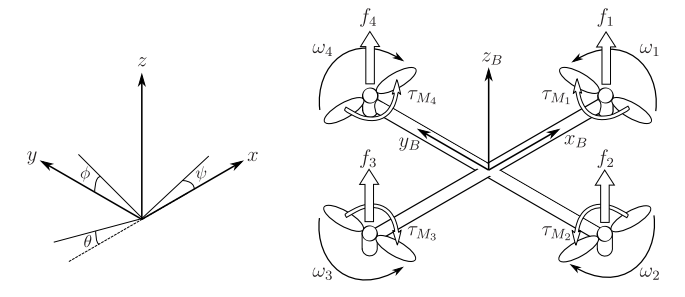
\includegraphics[width=\linewidth]{img/reference_frames.png}
  \caption{The inertial and body frames of a quadcopter using the East North Up convention (ENU). Figure from \cite{aalto}.}
  \label{fig:reference_frames}
\end{figure}

\subsection{Quadcopter Dynamics}
\label{ssec:dynamics}

The following derivations are a summary of the equations in \cite{aalto}.
\begin{itemize}
  \item The angular velocity of rotor $i,$ denoted with $\omega_{i},$ creates force $f_{i}$ in the direction of
the rotor axis: 
$$f_{i}=k \omega_{i}^{2}$$

where the lift constant is $k$.
The combined forces of rotors create thrust $T$ in the direction of the body z-axis (represented as $\boldsymbol{T}_{B}$).

$$T=\sum_{i=1}^{4} f_{i}=k \sum_{i=1}^{4} \omega_{i}^{2}, \quad \quad \boldsymbol{T}_{B}=\left[ \begin{array}{c}{0} \\ {0} \\ {T}\end{array}\right]$$

  \item The angular velocity and acceleration of the rotor also creates torque $\tau_{M_i}$ around the rotor axis: 
  $$I_{M} \dot{\omega}_{i} = \tau_{M_{i}} - b \omega_{i}^{2}$$
  in which the drag constant is $b$ and the inertia moment of the
rotor is $I_{M}$. 
Usually the acceleration of the rotor ($\dot{\omega}_{i}$) is considered small and thus it is omitted.
  This holds when we assume that the quadrotor is operating in stable flight and that the propellers are maintaining a constant thrust and not accelerating.
  This assumption results in the torque about the global z axis being equal to the torque due to drag.

Torque $\boldsymbol{\tau_B}$ consists of the torques on the three axis $\tau_\phi, \tau_\theta, \tau_\psi$:

$$
\boldsymbol{\tau}_{B}=\left[ \begin{array}{c}{\tau_{\phi}} \\ {\tau_{\theta}} \\ {\tau_{\psi}}\end{array}\right]=
\left[ \begin{array}{c}{l k\left(-\omega_{2}^{2}+\omega_{4}^{2}\right)} \\ {l k\left(-\omega_{1}^{2}+\omega_{3}^{2}\right)} \\ {\sum_{i=1}^{4} (-1)^{i+1} \tau_{M_{i}}}\end{array}\right]
  $$
  $$
  =
\left[ \begin{array}{c}
{l k\left(-\omega_{2}^{2}+\omega_{4}^{2}\right)} \\
{l k\left(-\omega_{1}^{2}+\omega_{3}^{2}\right)} \\
{b(\omega_{1}^{2}-\omega_{2}^{2}+\omega_{3}^{2}-\omega_{4}^{2})}\end{array}\right]
  $$

where $l$ is the distance between the rotor and the center of mass of the quadcopter.

\end{itemize}


\subsubsection{Translational dynamics}

Newton's second law: 
$$m \ddot{\boldsymbol{\xi}}=\boldsymbol{G}+\boldsymbol{R} \boldsymbol{T}_{B}$$

$$\left[ \begin{array}{c}{\ddot{x}} \\ {\ddot{y}} \\ {\ddot{z}}\end{array}\right]=-g \left[ \begin{array}{l}{0} \\ {0} \\ {1}\end{array}\right]+\frac{T}{m} \left[ \begin{array}{c}{C_{\psi} S_{\theta} C_{\phi}+S_{\psi} S_{\phi}} \\ {S_{\psi} S_{\theta} C_{\phi}-C_{\psi} S_{\phi}} \\ {C_{\theta} C_{\phi}}\end{array}\right]$$

\subsubsection{Rotational dynamics}
The rotational equations of motion are defined in the body frame so that the rotations can be computed about the quadrotor’s center and not the center of the global coordinate frame.
Applying Euler's second law:
$$\boldsymbol{I} \dot{\boldsymbol{\nu}}+\boldsymbol{\nu} \times(\boldsymbol{I} \boldsymbol{\nu})+\mathbf{\Gamma}=\boldsymbol{\tau}$$
where we have:
\begin{itemize}
  \item Angular acceleration of the inertia: $\boldsymbol{I\dot{v}}$
  \item Centripetal forces: $\boldsymbol{\nu}\times(\boldsymbol{I \nu})$
  \item Gyroscopic forces: $\boldsymbol{\Gamma}$
  \item External torque: $\boldsymbol{\tau}_B$
\end{itemize}

Replacing terms by their definitions, multiplying both sides by $\boldsymbol{I}^{-1}$, and rearranging:
$$\boldsymbol{\dot{\nu}}=\boldsymbol{I}^{-1}\left(-\left[ \begin{array}{c}{p} \\ {q} \\ {r}\end{array}\right] \times \left[ \begin{array}{c}{I_{x x} p} \\ {I_{y y} q} \\ {I_{z z} r}\end{array}\right]-I_{r} \left[ \begin{array}{c}{p} \\ {q} \\ {r}\end{array}\right] \times \left[ \begin{array}{c}{0} \\ {0} \\ {1}\end{array}\right] \omega_{\Gamma}+\boldsymbol{\tau}_B\right)$$

$$
\begin{array}{c}
\left[ \begin{array}{c}{\dot{p}} \\ {\dot{q}} \\ {\dot{r}}\end{array}\right]= 
\left[ \begin{array}{c}{\left(I_{y y}-I_{z z}\right) q r / I_{x x}} \\ {\left(I_{z z}-I_{x x}\right) p r / I_{y y}} \\ {(I_{x x}-I_{y y}) p q / I_{z z}}\end{array}\right] 
- I_{r} \left[ \begin{array}{c}{q / I_{x x}} \\ {-p / I_{y y}} \\ {0}\end{array}\right] \omega_{\Gamma} \\
+ \left[ \begin{array}{c}{\tau_{\phi} / I_{x x}} \\ {\tau_{\theta} / I_{y y}} \\ {\tau_{\psi} / I_{z z}}\end{array}\right]
\end{array}
  $$

  where $\omega_\Gamma = \omega_1 - \omega_2 + \omega_3 - \omega_4$, and $I_r$ is the rotor moment of inertia.


The angular accelerations $\ddot{\boldsymbol{\eta}}$ in world frame are given by the time derivatives of the angular velocities $\left(\dot{\boldsymbol{\eta}} = \boldsymbol{W}_{\eta}^{-1} \boldsymbol{\nu}\right)$,

$$\ddot{\boldsymbol{\eta}}=\frac{\mathrm{d}}{\mathrm{d} t}\left(\boldsymbol{W}_{\eta}^{-1} \boldsymbol{\nu}\right) =\frac{\mathrm{d}}{\mathrm{d} t}\left(\boldsymbol{W}_{\eta}^{-1}\right) \boldsymbol{\nu}+\boldsymbol{W}_{\eta}^{-1} \dot{\boldsymbol{\nu}} = $$

$$
\begin{array}{c}
\left[ \begin{array}{cccc}{0} & {\dot{\phi} C_{\phi} T_{\theta}+\dot{\theta} S_{\phi} / C_{\theta}^{2}} & {-\dot{\phi} S_{\phi} C_{\theta}+\dot{\theta} C_{\phi} / C_{\theta}^{2}} \\ {0} & {-\dot{\phi} S_{\phi}} & {-\dot{\phi} C_{\phi}} \\ {0} & {\dot{\phi} C_{\phi} / C_{\theta}+\dot{\phi} S_{\phi} T_{\theta} / C_{\theta}} & {-\dot{\phi} S_{\phi} / C_{\theta}+\dot{\theta} C_{\phi} T_{\theta} / C_{\theta}}\end{array}\right] \boldsymbol{\nu}
\\ + \boldsymbol{W_{\eta}^{-1}} \dot{\boldsymbol{\nu}}.
\end{array}
  $$

At this point, it is common to do a simplification by setting $[\dot{\phi} \quad \dot{\theta} \quad \dot{\psi}]^{T}=\left[ \begin{array}{lll}{p} & {q} & {r}\end{array}\right]^{T}$, which holds true for small angles of movement \cite{Sabatino2015}.
  Nevertheless, in this work we omit such a simplification.

\subsection{Aerodynamic Drag}
\label{ssec:drag}

  We include the drag force generated by the air resistance. For this, we add a diagonal coefficient matrix that associates the linear velocities to the force slowing down the movement

  $$
    \begin{array}{l}
      \left[ \begin{array}{l}{\ddot{x}} \\ {\ddot{y}} \\ {\ddot{z}}\end{array}\right]=-g \left[ \begin{array}{l}{0} \\ {0} \\ {1}\end{array}\right]+\frac{T}{m} \left[ \begin{array}{c}{C_{\psi} S_{\theta} C_{\phi}+S_{\psi} S_{\phi}} \\ {S_{\psi} S_{\theta} C_{\phi}-C_{\psi} S_{\phi}} \\ {C_{\theta} C_{\phi}}\end{array}\right] \\
      \quad \quad \quad \quad  - \frac{1}{m} \left[ \begin{array}{ccc}{A_{x}} & {0} & {0} \\ {0} & {A_{y}} & {0} \\ {0} & {0} & {A_{z}}\end{array}\right] \left[ \begin{array}{c}{\dot{x}} \\ {\dot{y}} \\ {\dot{z}}\end{array}\right]
    \end{array}
  $$

  in which $A_{x}, A_{y}$ and $A_{z}$ are the drag force coefficients for velocities in the corresponding directions of the inertial frame.
  Several other aerodynamical effects could be included in the model. For example,
dependence of thrust on angle of attack, blade flapping and airflow disruptions.
We refrain from adding these for simplicity of the model.
  We also ignore rotational drag forces since we assume rotational velocities to be small. Alternatively,
   we could add the components $\boldsymbol{\tau}_{\boldsymbol{w}}=\left[ \begin{array}{lll}{\tau_{w x}} & {\tau_{w y}} & {\tau_{w z}}\end{array}\right]^{T}$ to the overall torque.

\subsection{State-space Model}
\label{ssec:state_space_model}

We can write our nonlinear dynamics using the following state vector:

$\boldsymbol{X}^{T}=\left[\begin{array}{cccccccccccc}{x} & {y} & {z} & {\dot{x}} & {\dot{y}} & {\dot{z}} & {\phi} & {\theta} & {\psi} & {p} & {q} & {r}\end{array}\right]^{T}$

Moreover, we define our inputs as follow:
\begin{itemize}
  \item $U_1$: the resulting thrust of the four rotors.
  \item $U_2$: the difference of thrust between the motors on the $x$ axis which results in roll angle changes and subsequent movement in the lateral $x$ direction.
  \item $U_3$: the difference of thrust between the motors on the $y$ axis which results in pitch
  angle changes and subsequent movement in the lateral $y$ direction.
  \item $U_4$: the difference of torque between the clockwise and counterclockwise rotors which
  results in a moment that rotates the quadrotor around the vertical $z$ axis.
\end{itemize}

This results in the control vector $U$ defined as:
$$U=\left[ \begin{array}{l}{U_{1}} \\ {U_{2}} \\ {U_{3}} \\ {U_{4}}\end{array}\right]= \left[ \begin{array}{c}{T} \\ {\tau_{\phi}} \\ {\tau_{\theta}} \\ {\tau_{\psi}}\end{array}\right]=
\left[ \begin{array}{c}
{k \sum_{i=1}^{4} \omega_{i}^{2}} \\
{l k\left(-\omega_{2}^{2}+\omega_{4}^{2}\right)} \\ 
{l k\left(-\omega_{1}^{2}+\omega_{3}^{2}\right)} \\ 
{b(\omega_{1}^{2}-\omega_{2}^{2}+\omega_{3}^{2}-\omega_{4}^{2})}\end{array}\right]
.$$

Our nonlinear dynamics can be written as a nonlinear differential equation of the states $\boldsymbol{X}$ and control inputs $\boldsymbol{U}$:
\begin{equation}
  \label{eq:dynamics}
  \dot{\boldsymbol{X}}=f(\boldsymbol{X}, \boldsymbol{U}).
\end{equation}

Or, more precisely:
$$
\dot{\boldsymbol{X}} = 
\left[
\begin{array}{c}
\dot{x} \\
{}\\
\dot{y} \\
{}\\
\dot{z} \\
{}\\
{}\\
\ddot{x} \\
{}\\
\ddot{y} \\
{}\\
\ddot{z} \\
{}\\
{}\\
\dot{\phi} \\
{}\\
\dot{\theta} \\
{}\\
\dot{\psi} \\
{}\\
{}\\
\dot{p} \\
{}\\
\dot{q} \\
{}\\
\dot{r}
\end{array}
\right]
=
\left[
\begin{array}{l}

\dot{x} \\
{}\\
\dot{y} \\
{}\\
\dot{z} \\
{}\\
{}\\
  \frac{T}{m}[S_{\phi} S_{\psi}+C_{\phi} C_{\psi} S_{\theta}] - \frac{A_x}{m} \dot{x} \\
{}\\
  \frac{T}{m}[C_{\phi} S_{\psi} S_{\theta}-C_{\psi} S_{\phi}] - \frac{A_y}{m} \dot{y} \\
{}\\
  -g+\frac{T}{m}[C_{\phi} C_{\theta}] - \frac{A_z}{m} \dot{z} \\
{}\\
{}\\
  p+r[C_{\phi} T_{\theta}]+q[S_{\phi} T_{\theta}] \\
{}\\
  q[C_{\phi}]-r[S_{\phi}] \\
{}\\
  r \frac{C_{\phi}}{C_{\theta}}+q \frac{S_{\phi}}{C_{\theta}} \\
{}\\
{}\\
\frac{I_{y}-I_{z}}{I_{x}} r q - \frac{I_r}{I_{x}} q w_{\Gamma} +\frac{\tau_{\phi}}{I_{x}} \\
{}\\
\frac{I_{z}-I_{x}}{I_{y}} p r + \frac{I_r}{I_{y}} p w_{\Gamma} +\frac{\tau_{\theta}}{I_{y}} \\
{}\\
\frac{I_{x}-I_{y}}{I_{z}} p q +\frac{\tau_{\psi}}{I_{z}}
\end{array}
\right]
=f(\boldsymbol{X}, \boldsymbol{U})
$$

\section{Minimum Time Optimal Control Problem}
\label{ssec:optimization_problem}

A P-phase optimal control problem can be stated in the following general form.
 Determine the state
$\mathbf{x}^{(p)}(t) \in \mathbb{R}^{n(p)},$ control, $\mathbf{u}^{(p)}(t) \in \mathbb{R}^{n(t)},$ initial time, $t_{0}^{(p)} \in \mathbb{R},$ final time, $t_{f}^{(p)} \in \mathbb{R},$
in each phase $p \in[1, \ldots, P],$ that minimize a given cost functional, subject to dynamic constraints:
$$\dot{\mathbf{x}}^{(p)}=\mathbf{a}^{(p)}\left[\mathbf{x}^{(p)}, \mathbf{u}^{(p)}, t^{(p)}\right], \quad(p=1, \ldots, P)$$

\textbf{Cost}: our objective is to minimize the time taken for the drone to pass through all gates in a particular order.
Therefore, the cost we try to minimize is simply the final time:

$$J= \sum_{p}\int_{t^{(p)}_0}^{t^{(p)}_f} d t =\int_{t_{0}}^{t_{f}} d t = t_f$$
where $t_0 = 0$ is fixed, but $t_f$ is free.
We consider that the drone has finished the race once it has reached the last gate.

\textbf{Nonlinear Dynamics:} are formulated using the generic form: $\dot{x}(t)= f(x(t), u(t), t).$
As detailed in \cref{eq:dynamics}, we make use of a nonlinear function of the state $\boldsymbol{X}(t)$ and the input $\boldsymbol{U}(t)$.
Although the nonlinear function $f$ may depend explicitly on time $t$, the drone dynamics do not depend directly on $t$, therefore the time dependency can be dropped.

\textbf{Phases:}
the racetrack is constructed in a piecewise fashion using phases, where each phase spans from one gate to the next one.
Therefore, we consider as many phases as there are gates in the racetrack.

\textbf{Bounds:} to simulate a realistic drone we must constraint the control inputs to a range of possible values.
\begin{itemize}
  \item Input Bounds: generic input constraints can be formulated as: 
  $$M_{i}^{-} \leq U_{i}(t) \leq M_{i}^{+},$$
  where $M_{i}^{-}$ is the lower bound of control input $U_{i}(t)$, while $M_{i}^{+}$ is its upper bound.
  In our case, we use the bounds in \cref{tab:control_bounds}, which were calculated using the following heuristics.
  For bounds on $U_1$ input (thrust) the minimum bound is $0$ since we consider that the quadcopter has fixed-pitch propellers.
  With a variable pitch propeller, one may expect the thrust to be negative as well.
  The upper bound is calculated as $4 k \omega_{\text{max}}^{2}$, where $k$ is the lift constant and $\omega_{\text{max}}$ is the maximum motor speed.
  For $U_2, U_3$ upper and lower bounds we use $\pm 4 k l \omega_{\text{max}}^{2}$, where $l$ is the quadrotor's arm length.
  Similarly, for the yaw component $U_4$, we use  $\pm 2 k l \omega_{\text{max}}^{2}$.
  \begin{table}[htbp]
    \center
    \begin{tabular}{|c|c|c|c|}
      \hline 
      Input & Definition & $M_i^{-}$ & $M_i^{+}$ \\
      \hline 
      {$U_1$} & {Thrust} & 0.0 & 43.5 \\
      {$U_2$} & {Roll rate} & -6.25 & 6.25 \\
      {$U_3$} & {Pitch rate} & -6.25 & 6.25\\
      {$U_4$} & {Yaw rate} & -2.25 & 2.25\\
      \hline
    \end{tabular}
    \caption{Constraints on control inputs.}
    \label{tab:control_bounds}
  \end{table}
%  Quad.U1_max = 43.5;   % Quad.KT*4*Quad.max_motor_speed^2
%Quad.U1_min = 0;      %
%Quad.U2_max = 6.25;  % Quad.KT*Quad.l*Quad.max_motor_speed^2
%Quad.U2_min = -6.25; % Quad.KT*Quad.l*Quad.max_motor_speed^2
%Quad.U3_max = 6.25;  % Quad.KT*Quad.l*Quad.max_motor_speed^2
%Quad.U3_min = -6.25; % Quad.KT*Quad.l*Quad.max_motor_speed^2
%Quad.U4_max = 2.25; % Quad.Kd*2*Quad.max_motor_speed^2
%Quad.U4_min = -2.25;% Quad.Kd*2*Quad.max_motor_speed^2

  \item State Constraints: 

\end{itemize}

\textbf{Boundary Conditions:}

Given 
\begin{itemize}
  \item Initial: $n(x(t_{0}), t_{0}) = 0$
  \item Final: $m(x(t_{f}), t_{f}) = 0$
\end{itemize}

\textbf{Initial Conditions}
